\begin{titlepage}
% Strona tytułowa
\vbox to\textheight{\hyphenpenalty=10000
\begin{center}
	\begin{tabular}{p{10cm} p{30cm}}
		\begin{minipage}{10cm}
			\begin{center}
				\ \\
				\ \\
				Politechnika Warszawska \\
				Wydział Elektroniki i Technik Informacyjnych \\
				Instytut Informatyki
			\end{center}
		\end{minipage}
		&
		\begin{minipage}{12cm}
			\begin{flushleft}
				\footnotesize
				Rok akademicki 2015/2016
				\vspace*{2.75\baselineskip}
			\end{flushleft}
		\end{minipage} \\
		\vspace*{1.0\baselineskip}
	\end{tabular}
	
\includegraphics[width=4cm]{img/logo_pw2}
	\par\vspace{\smallskipamount}
	\vspace*{2\baselineskip}{\LARGE PRACA DYPLOMOWA MAGISTERSKA\par}
	\vspace{3\baselineskip}{\LARGE\strut Krzysztof Lis\par}
	\vspace*{2\baselineskip}{\huge\bfseries Projekt systemu wspomagającego ocenę ryzyka kredytowego \\w oparciu o dane historyczne\par}
	\vspace*{4\baselineskip}
	\hfill\mbox{}\par\vspace*{\baselineskip}\noindent
	
	\begin{tabular}[b]{@{}p{3cm}@{\ }l@{}}
		{\large\hfill } & {\large }
	\end{tabular}
	\hfill
	\begin{tabular}[b]{@{}l@{}}
		Opiekun pracy: \\[\smallskipamount]
		{\large dr inż. Andrzej Ciemski}
	\end{tabular}\par
	\vspace*{1\baselineskip}
	\begin{tabular}{p{\textwidth}}
		\begin{flushleft}
			\begin{minipage}{7cm}
				Ocena \dotfill
				\par\vspace{1.6\baselineskip}
				\dotfill
				\par\noindent
				\centerline{\footnotesize Podpis Przewodniczącego} \par
				\centerline{\footnotesize Komisji Egzaminu Dyplomowego}\par
			\end{minipage}
		\end{flushleft}
	\end{tabular}
\end{center}}

% Życiorys
\newpage\thispagestyle{empty}
\begin{tabular}{p{4cm} p{9cm}}
	\begin{minipage}{4cm}
		\begin{flushleft}
			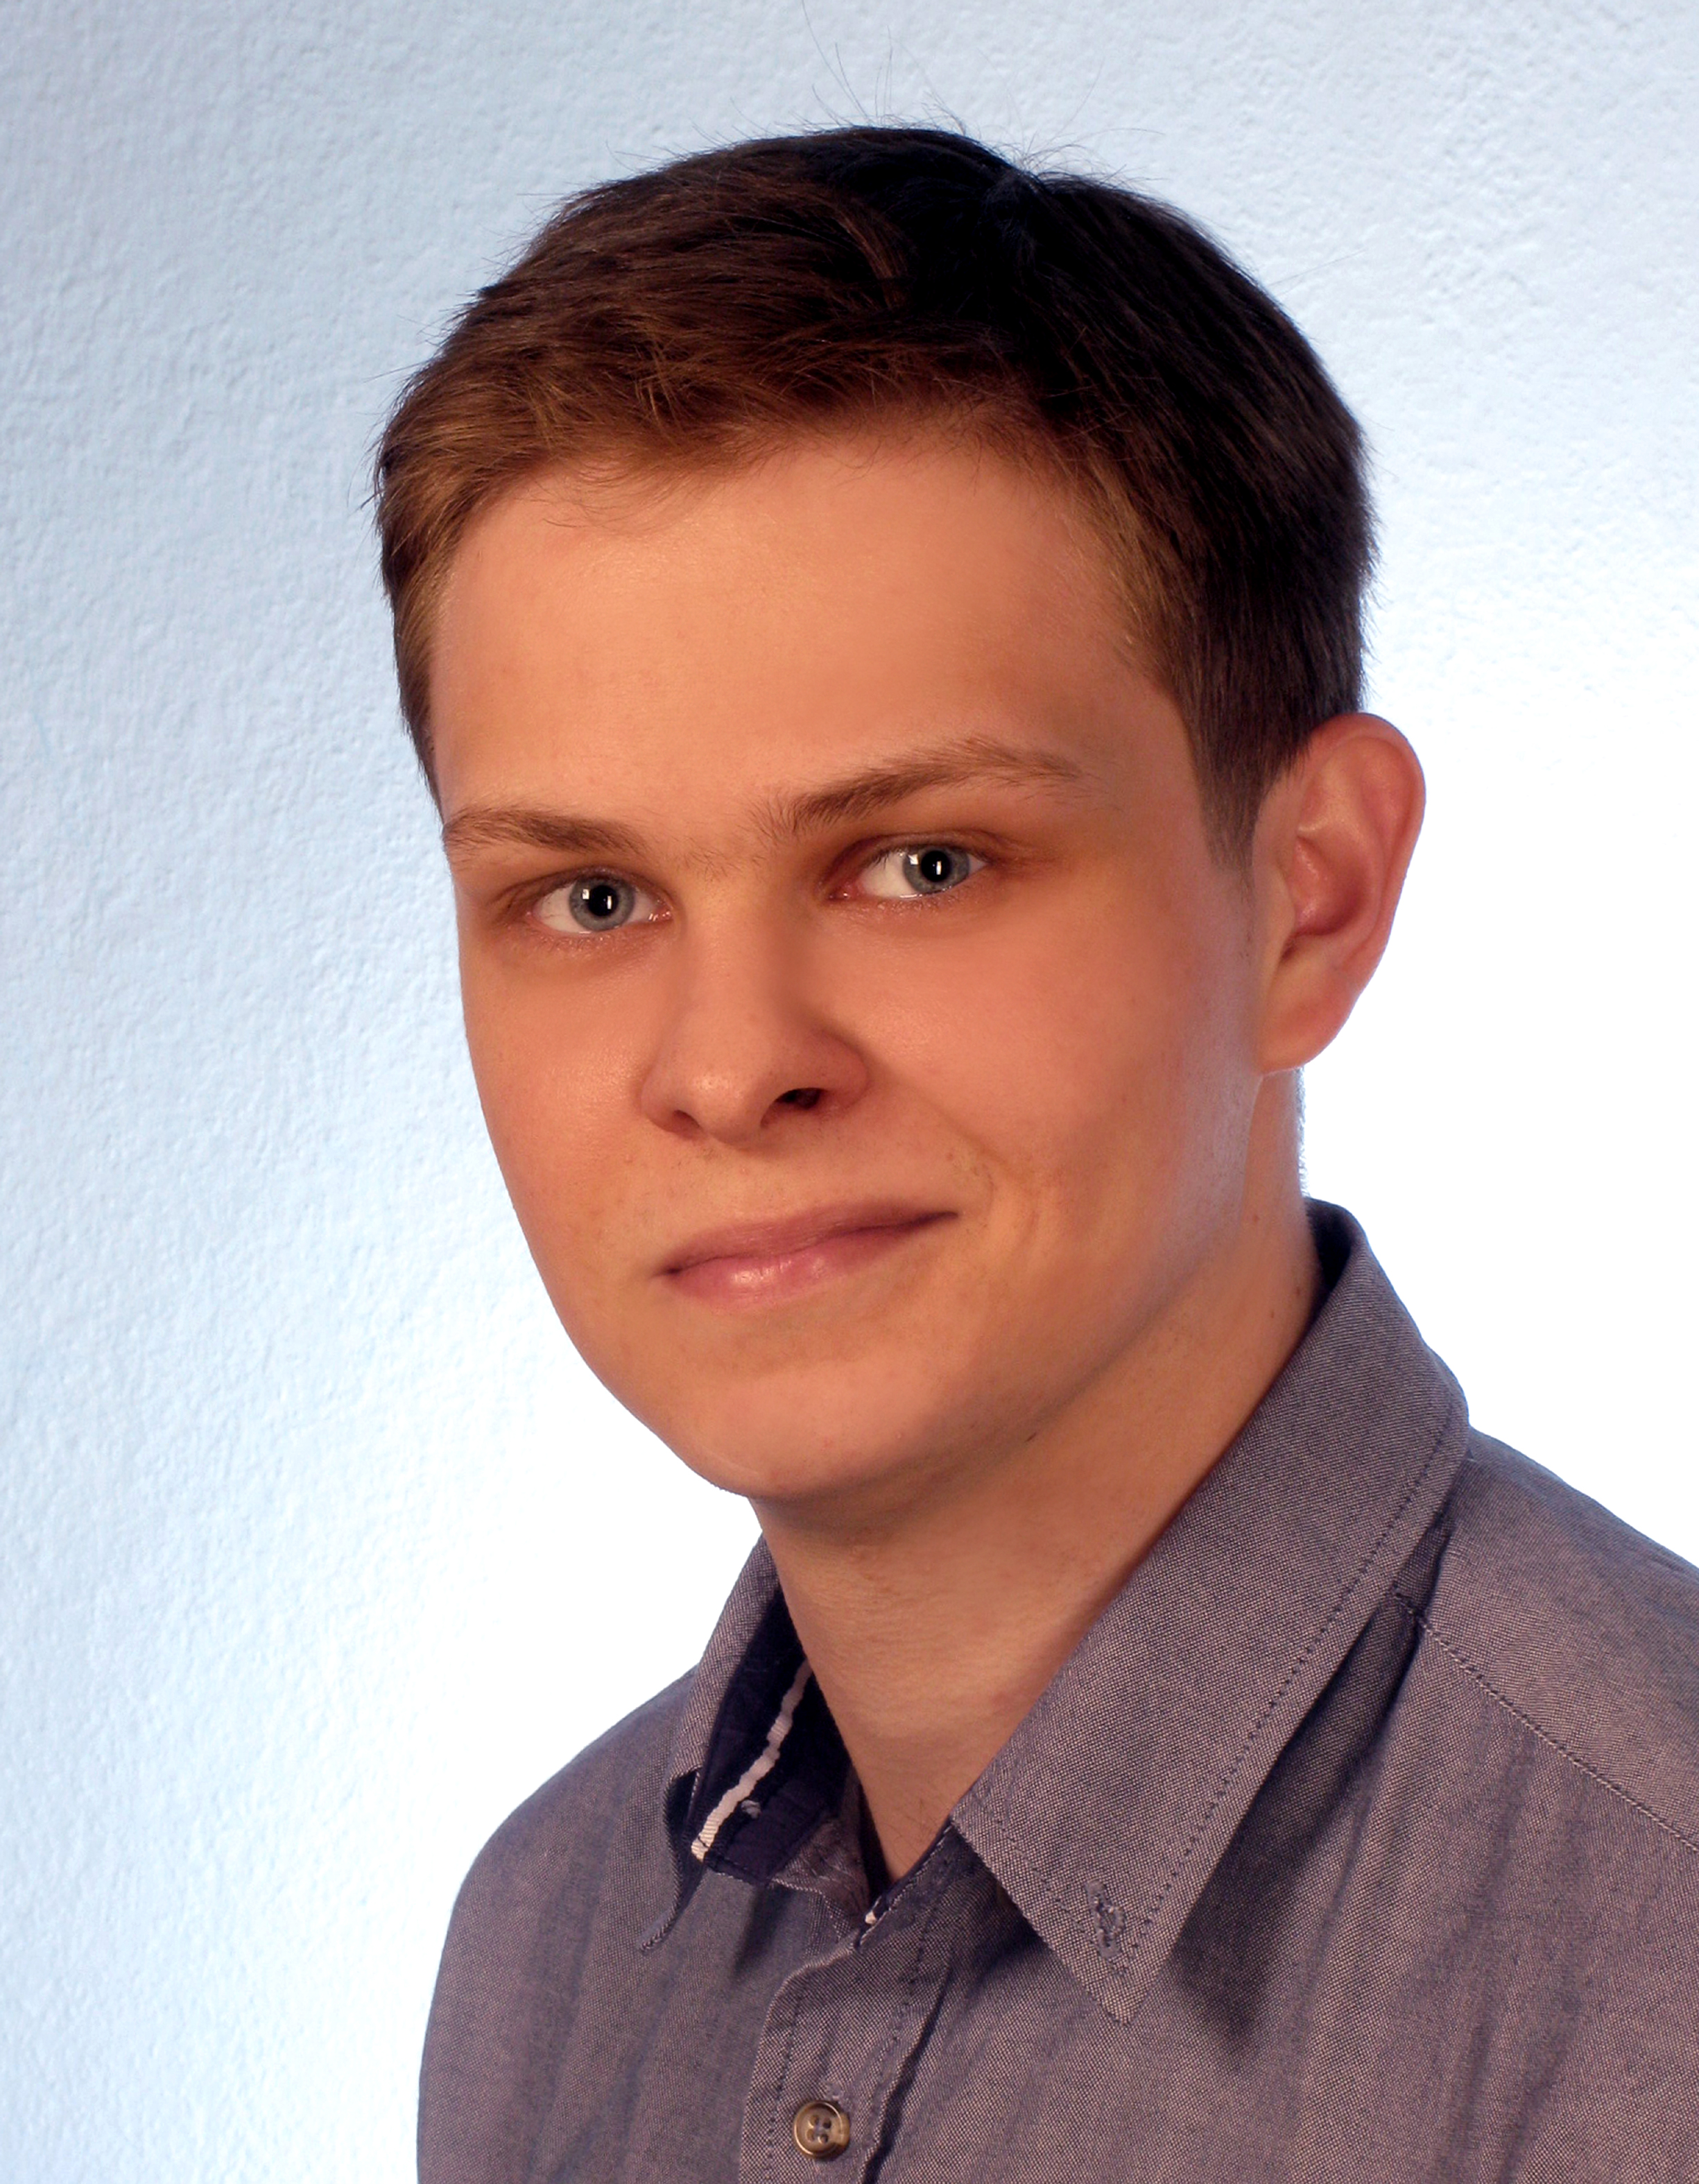
\includegraphics[height=5.0cm,width=4.0cm]{img/profile.jpg}
		\end{flushleft}
	\end{minipage}
	&
	\begin{minipage}{12cm}
		\begin{flushleft}
			\par\noindent\vspace{1\baselineskip}
			\begin{tabular}[h]{l r}
				{\normalsize\it Kierunek:} & \ \ \ \ \ \ \ \ \ \ \ \ \ \ \ \ \ \ \ \ \ \ \ \ \ \ \ \ \ \ \ \ \ \ \ \ \ \ \ \ \ \ \ Informatyka
			\end{tabular}
			\par\noindent\vspace{1\baselineskip}
			\begin{tabular}[h]{l r}
				{\normalsize\it Specjalność:} & Inżynieria Systemów Informatycznych
			\end{tabular}
			\par\noindent\vspace{1\baselineskip}
			\begin{tabular}[h]{l r}
				{\normalsize\it Data rozpoczęcia studiów:} & {\normalsize \ \ \ \ \ \ \ \ \ \ \ \ \ \ \ \ \ 24.02.2014 r.}
			\end{tabular}
			\par\noindent\vspace{1\baselineskip}
		\end{flushleft}
	\end{minipage}
\end{tabular}

\vspace*{1\baselineskip}
\begin{center}
{\large\bfseries Życiorys}\par\bigskip
\end{center}

\indent
Nazywam się Krzysztof Lis. Urodziłem się 19 czerwca 1991 roku w Nowym Jorku. W 2010 roku rozpocząłem studia na Wydziale Mechatroniki Politechniki Warszawskiej na kierunku Automatyka i Robotyka. I stopień studiów skończyłem na specjalności Automatyka z wyróżnieniem ``Summa Cum Laude'' przyznawanym przez Rektora Politechniki Warszawskiej. W ramach pracy inżynierskiej współpracowałem z firmą Siemens nad robotyzacją procesu paletyzacji. Podczas pracy nad projektem jako pierwszy w Polsce wykorzystałem środowisko Tecnomatix RobotExpert® wprowadzone przez firmę Siemens. Po uzyskaniu tytułu inżyniera rozpocząłem studia II stopnia na Wydziale Elektroniki i Technik Informacyjnych na kierunku Informatyka. W trakcie studiów pracowałem w warszawskim start-upie projektującym system dla centrum obrabiarkowego oraz rozpocząłem pracę jako programista w dziale technologii banku inwestycyjnego Goldman Sachs, gdzie miałem okazję brać udział w projektach prowadzonych w Polsce, Stanach Zjednoczonych oraz Wielkiej Brytanii.
\par
\vspace{2\baselineskip}
\hfill\parbox{15em}{{\small\dotfill}\\[-.3ex]
\centerline{\footnotesize podpis studenta}}\par
\vspace{3\baselineskip}
\begin{center}
	{\large\bfseries Egzamin dyplomowy} \par\bigskip\bigskip
\end{center}
\par\noindent\vspace{1.5\baselineskip}
Złożył egzamin dyplomowy w dniu \dotfill 20\_\_r.
\par\noindent\vspace{1.5\baselineskip}
z wynikiem \dotfill
\par\noindent\vspace{1.5\baselineskip}
Ogólny wynik studiów \dotfill
\par\noindent\vspace{1.5\baselineskip}
Dodatkowe wnioski i uwagi Komisji \dotfill
\par\noindent\vspace{1.5\baselineskip}
\dotfill



% Streszczenie
\newpage\thispagestyle{empty}
\vspace*{2\baselineskip} 
\begin{center}
	{\large\bfseries Streszczenie}\par\bigskip
\end{center}

{\itshape
Celem pracy magisterskiej jest omówienie teorii zagadnienia oceny ryzyka kredytowego w oparciu o dane historyczne. Przeprowadzono analizę danych pochodzących z platformy Lending Club®, na podstawie której dobrano model uczenia maszynowego obliczający prawdopodobieństwo niespłacenia pożyczki w oparciu o dane historyczne. Wybrany model został wykorzystany jako komponent przykładowej aplikacji web'owej umożliwiającej użytkownikowi przegląd statystyk pożyczek oraz ocenę ryzyka kredytowego dla danej pożyczki. W celu poprawy skalowalności aplikacji, uniezależnienia jej od środowiska w jakim jest uruchamiana oraz przystosowania do pracy w chmurze wykorzystano technologię kontenerów aplikacyjnych. 
}
\vspace*{1\baselineskip}

\noindent{\bf Słowa kluczowe}: {\itshape web, kontenery aplikacyjne, ryzyko kredytowe, systemy wspomagające podejmowanie decyzji, machine learning}
\par
\vspace{4\baselineskip}
\begin{center}
	{\large\bfseries The design of the web application supporting credit risk evaluation based on historic data.}\par\bigskip
\end{center}

{\itshape
This thesis picks up on the topic of the credit risk evaluation based on historic data. The author conducted a thorough analysis of data published by Lending Club in order to select an appropriate machine learning model, that would estimate the probability of default for a given loan. This component became the core of a sample web application, that allows users to view loan statistics and assess the credit risk of a particular loan. The scalability, environment isolation and cloud-compatibility issues were addressed by incorporating the application containers technology into the project.}
\vspace*{1\baselineskip}

\noindent{\bf Keywords}: {\itshape web, application containers, credit risk, decision support systems, machine learning}

\end{titlepage}